\documentclass[aspectratio=169, 10pt]{beamer}

% --- GÓI TIẾNG VIỆT VÀ ĐỊNH DẠNG ---
\usepackage[T5]{fontenc}
\usepackage[utf8]{inputenc}
\usepackage[vietnamese]{babel}
\usepackage{amsmath, amssymb, amsfonts}
\usepackage{graphicx}
\usepackage{booktabs, multirow, array}
\usepackage{xcolor}
\usepackage{tikz}
\usetikzlibrary{calc, shapes.geometric, arrows.meta, positioning, shadows}

% --- BẢNG MÀU NHẬN DIỆN THƯƠNG HIỆU HCMUE (Chuẩn theo Mau sac chu dao.png) ---
\definecolor{HCMUEDarkBlue}{RGB}{18, 72, 116}    % #124874 (Xanh ĐH Sư Phạm TP.HCM)
\definecolor{HCMUERed}{RGB}{207, 55, 61}        % #CF373D (Đỏ ĐH Sư Phạm TP.HCM)
\definecolor{HCMUECerulean}{RGB}{2, 132, 199}   % #0284C7 (Xanh da trời công nghệ)
\definecolor{HCMUEGold}{RGB}{217, 119, 6}       % #D97706 (Vàng hổ phách điểm nhấn)
\definecolor{HCMUELightBlue}{RGB}{241, 247, 254}% Nền khối dịu mắt
\definecolor{HCMUEDarkText}{RGB}{30, 41, 59}    % Slate 800
\definecolor{HCMUEGray}{RGB}{100, 116, 139}     % Slate 500
\definecolor{HCMUEGreen}{RGB}{22, 163, 74}      % Xanh lá tích cực

% --- THIẾT LẬP GIAO DIỆN BEAMER ---
\useinnertheme{rounded}
\useoutertheme{infolines}
\setbeamersize{text margin left=0.6cm, text margin right=0.6cm}
\setbeamertemplate{navigation symbols}{}

\setbeamercolor{palette primary}{bg=HCMUEDarkBlue, fg=white}
\setbeamercolor{palette secondary}{bg=HCMUEDarkBlue!90!black, fg=white}
\setbeamercolor{palette tertiary}{bg=HCMUEDarkBlue!80!black, fg=white}
\setbeamercolor{palette quaternary}{bg=HCMUEDarkBlue!70!black, fg=white}

\setbeamercolor{structure}{fg=HCMUEDarkBlue}
\setbeamercolor{titlelike}{parent=palette primary, fg=HCMUEDarkBlue}
\setbeamercolor{frametitle}{bg=white, fg=HCMUEDarkBlue}
\setbeamercolor{normal text}{fg=HCMUEDarkText, bg=white}
\setbeamercolor{item}{fg=HCMUEDarkBlue}
\setbeamercolor{subitem}{fg=HCMUERed}

% Định dạng Block
\setbeamercolor{block title}{bg=HCMUEDarkBlue, fg=white}
\setbeamercolor{block body}{bg=HCMUELightBlue, fg=HCMUEDarkText}

\setbeamercolor{block title example}{bg=HCMUECerulean, fg=white}
\setbeamercolor{block body example}{bg=HCMUELightBlue!60!white, fg=HCMUEDarkText}

\setbeamercolor{block title alerted}{bg=HCMUERed, fg=white}
\setbeamercolor{block body alerted}{bg=HCMUERed!8!white, fg=HCMUEDarkText}

\setbeamertemplate{blocks}[rounded][shadow=true]

% Hình nền mờ Tòa nhà A-01 chuẩn theo slide mẫu HCMUE_PPT Template.pptx
\setbeamertemplate{background}{%
  \begin{tikzpicture}[remember picture, overlay]
    \node[anchor=south east, inner sep=0pt] at ($(current page.south east)+(0, 0.35cm)$) {%
      
\includegraphics[width=8.5cm]{images/toa_nha_a_watermark_content.png}%
    };
  \end{tikzpicture}%
}

% Header (Frametitle) đồng bộ nhận diện thương hiệu HCMUE nguyên bản
\setbeamertemplate{frametitle}{%
  \nointerlineskip%
  \begin{beamercolorbox}[wd=\paperwidth,ht=0.96cm,dp=0.16cm]{frametitle}%
    \vbox to 0.96cm{%
      \vfill%
      \hbox to \paperwidth{%
        \hspace{0.55cm}%
        \parbox[c]{0.68\paperwidth}{\fontsize{10.5}{12.5}\selectfont\textbf{\color{HCMUEDarkBlue}\insertframetitle}}%
        \hfill%
        
\includegraphics[height=0.50cm,keepaspectratio]{images/logo_hcmue_kemchu_eng.png}%
        \hspace{0.55cm}%
      }%
      \vfill%
    }%
  \end{beamercolorbox}%
  \nointerlineskip%
  {\color{HCMUERed}\hrule height 1.8pt}%
  \vspace{0.18cm}%
}

% Footer (Footline)
\setbeamertemplate{footline}{%
  \leavevmode%
  {\color{HCMUERed}\hrule height 0.8pt}%
  \hbox{%
    \begin{beamercolorbox}[wd=.333333\paperwidth,ht=2.3ex,dp=1ex,leftskip=0.8cm]{palette primary}%
      \usebeamerfont{author in head/foot}\textbf{Nhập Môn NLP} — Nhóm 3 (KHMT K36)%
    \end{beamercolorbox}%
    \begin{beamercolorbox}[wd=.416667\paperwidth,ht=2.3ex,dp=1ex,center]{palette secondary}%
      \usebeamerfont{title in head/foot}\textbf{Từ Word2Vec đến BiLSTM \& Cơ Chế Attention}%
    \end{beamercolorbox}%
    \begin{beamercolorbox}[wd=.25\paperwidth,ht=2.3ex,dp=1ex,rightskip=0.8cm,right]{palette primary}%
      \usebeamerfont{date in head/foot}\textbf{HCMUE} $\mid$ \insertframenumber{} / \inserttotalframenumber%
    \end{beamercolorbox}%
  }%
  \vskip0pt%
}

% --- THÔNG TIN BÀI GIẢNG ---
\title[Nhập Môn Hiểu Ngôn Ngữ Tự Nhiên]{BÀI GIẢNG NHẬP MÔN XỬ LÝ NGÔN NGỮ TỰ NHIÊN}
\subtitle{TỪ VECTOR HÓA WORD2VEC ĐẾN MẠNG HỒI QUY LSTM VÀ CƠ CHẾ ATTENTION}

\author[Huy, Ngân, Phát]{
  \textbf{Giảng viên hướng dẫn: PGS.TS. LÊ ANH CƯỜNG}\\[0.3em]
  \textbf{Nhóm báo cáo viên (Cao học KHMT K36):}\\
  Trần Gia Huy $\bullet$ Đỗ Minh Khánh Ngân $\bullet$ Nguyễn Tấn Phát
}

\institute[HCMUE]{
  \textbf{TRƯỜNG ĐẠI HỌC SƯ PHẠM THÀNH PHỐ HỒ CHÍ MINH}\\
  \textbf{KHOA CÔNG NGHỆ THÔNG TIN — CAO HỌC KHOA HỌC MÁY TÍNH K36}
}

\date{Tháng 10 Năm 2026}

\begin{document}

% ==================== SLIDE 1: TRANG TIÊU ĐỀ BÀI GIẢNG ====================
{
\setbeamertemplate{background}{}
\setbeamertemplate{footline}{}
\setbeamertemplate{frametitle}{}
\begin{frame}[plain]
  \begin{tikzpicture}[remember picture,overlay]
    % Viền trên màu xanh đậm
    \fill[HCMUEDarkBlue] (current page.north west) rectangle ($(current page.north east)+(0,-0.10cm)$);
    % Dải banner màu trắng chứa logo kèm chữ nguyên bản
    \fill[white] ($(current page.north west)+(0,-0.10cm)$) rectangle ($(current page.north east)+(0,-1.55cm)$);
    
    % Logo kèm chữ chính thức từ folder "Logo kèm chữ" (Huy hiệu + Tên trường tiếng Việt & tiếng Anh)
    \node[anchor=west] at ($(current page.north west)+(0.8cm,-0.82cm)$) {
      
\includegraphics[height=0.92cm]{images/logo_hcmue_kemchu_eng.png}
    };
    
    % Đường phân cách màu đỏ chuẩn thương hiệu #CF373D và xanh
    \fill[HCMUERed] ($(current page.north west)+(0,-1.55cm)$) rectangle ($(current page.north east)+(0,-1.61cm)$);
    \fill[HCMUEDarkBlue] ($(current page.north west)+(0,-1.61cm)$) rectangle ($(current page.north east)+(0,-1.64cm)$);

    % Nền mờ Tòa nhà A-01 chuẩn phong cách HCMUE_PPT Template.pptx
    \node[anchor=south east, inner sep=0pt] at ($(current page.south east)+(0, 0)$) {
      
\includegraphics[width=9.5cm]{images/toa_nha_a_watermark_dark.png}
    };
  \end{tikzpicture}

  \vspace{0.95cm}
  \begin{center}
    {\fontsize{9.5}{11}\selectfont \textbf{\color{HCMUECerulean}BÀI GIẢNG CHUYÊN ĐỀ DÀNH CHO NGƯỜI MỚI BẮT ĐẦU (TỪ CON SỐ 0)}}\\[0.3em]
    {\fontsize{13}{16}\selectfont \textbf{\color{HCMUEDarkBlue}LÀM THẾ NÀO MÁY TÍNH HIỂU ĐƯỢC NGÔN NGỮ CON NGƯỜI?}}\\[0.25em]
    {\fontsize{9}{11}\selectfont \color{HCMUEGray}Khám phá Từ Vector Hóa Word2Vec, Mạng Nơ-ron Chuỗi LSTM đến Cơ Chế Attention}
  \end{center}

  \vspace{0.15cm}
  \begin{columns}[T, onlytextwidth]
    \begin{column}{0.48\textwidth}
      \begin{block}{\small\textbf{Thông Tin Học Phần \& Đơn Vị}}
        \fontsize{8}{10.5}\selectfont
        \textbf{Học phần}: Xử lý ngôn ngữ tự nhiên (NLP)\\
        \textbf{Đơn vị}: Trường ĐH Sư phạm TP.HCM (HCMUE)\\
        \textbf{Giảng viên hướng dẫn}: \textbf{\color{HCMUEDarkBlue}PGS.TS. LÊ ANH CƯỜNG}\\
        \textbf{Mục tiêu}: Dễ hiểu, trực quan, giải thích bản chất cốt lõi
      \end{block}
    \end{column}
    \hfill
    \begin{column}{0.48\textwidth}
      \begin{block}{\small\textbf{Người Trình Bày (Nhóm 3 Học Viên)}}
        \fontsize{8}{10.5}\selectfont
        1. \textbf{Trần Gia Huy} — MSHV: \textbf{KHMT836012}\\
        2. \textbf{Đỗ Minh Khánh Ngân} — MSHV: \textbf{KHMT836019}\\
        3. \textbf{Nguyễn Tấn Phát} — MSHV: \textbf{KHMT836026}\\
        \textbf{Thực hành tương tác}: \url{http://localhost:8501}
      \end{block}
    \end{column}
  \end{columns}
\end{frame}
}

% ==================== SLIDE 2: LỘ TRÌNH BÀI HỌC ====================
\begin{frame}{Lộ Trình Khám Phá: 6 Nấc Thang Nhận Thức}
  \begin{columns}[T, onlytextwidth]
    \begin{column}{0.48\textwidth}
      \begin{enumerate}
        \setlength{\itemsep}{0.7em}
        \item \textbf{\color{HCMUEDarkBlue}Câu hỏi khởi đầu}: Tại sao máy tính không đọc được chữ?
        \item \textbf{\color{HCMUEDarkBlue}Cách làm cổ điển}: One-Hot và Đếm từ (BoW / TF-IDF) gặp cạm bẫy gì?
        \item \textbf{\color{HCMUEDarkBlue}Cuộc cách mạng Word2Vec}: Khi từ ngữ trở thành các tọa độ hình học trong không gian.
      \end{enumerate}
    \end{column}
    \hfill
    \begin{column}{0.48\textwidth}
      \begin{enumerate}
        \setcounter{enumi}{3}
        \setlength{\itemsep}{0.7em}
        \item \textbf{\color{HCMUEDarkBlue}Từ từ đơn đến cả câu}: Tại sao phép cộng trung bình bị hỏng bởi chữ \textit{''không''}?
        \item \textbf{\color{HCMUEDarkBlue}Mạng nơ-ron LSTM}: Ba lô trí nhớ thông minh biết quên chuyện cũ, nạp chuyện mới.
        \item \textbf{\color{HCMUEDarkBlue}Cơ chế Attention}: Cây bút dạ quang giúp AI biết từ nào là chìa khóa cảm xúc.
      \end{enumerate}
    \end{column}
  \end{columns}

  \vspace{0.25cm}
  \begin{alertblock}{Phương châm bài giảng}
    \centering\fontsize{8}{10.5}\selectfont
    \textbf{Không lạm dụng công thức phức tạp — Tập trung vào trực giác toán học, ví dụ đời thực và ứng dụng!}
  \end{alertblock}
\end{frame}

% ==================== PHẦN 1: BẢN CHẤT MÁY TÍNH VỚI CHỮ ====================
\begin{frame}{1. Câu Hỏi Khởi Đầu: Tại Sao Máy Tính Không Đọc Được Chữ?}
  \begin{columns}[T, onlytextwidth]
    \begin{column}{0.48\textwidth}
      \begin{block}{Thực tế về máy tính}
        \fontsize{7.5}{9.5}\selectfont
        \begin{itemize}\setlength{\itemsep}{0.15em}
          \item Máy tính chỉ biết tính toán trên \textbf{con số thực} (cộng, trừ, nhân ma trận).
          \item Đối với máy tính, câu \textit{''Trường Sư Phạm rất đẹp''} chỉ là các mã Unicode nhị phân (\texttt{010101...}).
          \item Máy tính không có trực giác thế nào là \textit{''đẹp''}, thế nào là \textit{''xấu''}.
        \end{itemize}
      \end{block}
      \vspace{0.15cm}
      \begin{exampleblock}{Mục tiêu của Biểu diễn từ}
        \fontsize{7.5}{9.5}\selectfont
        Tìm chiếc \textbf{cầu nối toán học} biến mỗi từ thành vector: \textit{Các từ có nghĩa tương tự nhau sẽ có các vector nằm gần nhau!}
      \end{exampleblock}
    \end{column}
    \hfill
    \begin{column}{0.48\textwidth}
      \begin{alertblock}{Cách tiếp cận ngây thơ: Đánh số thứ tự (ID)}
        \fontsize{7.5}{9.5}\selectfont
        Giả sử đánh số từ điển:
        \textit{mèo} = $1$, \textit{chó} = $2$, \textit{xe\_tải} = $3$.
        \vspace{0.1cm}
        \textbf{Cạm bẫy toán học xuất hiện}:
        \begin{itemize}\setlength{\itemsep}{0.15em}
          \item Máy tính hiểu: $1 + 2 = 3$ $\implies$ \textit{Mèo + Chó = Xe tải} (?!)
          \item Khoảng cách giữa \textit{Mèo} và \textit{Xe tải} ($3 - 1 = 2$) lớn hơn khoảng cách \textit{Mèo} và \textit{Chó} ($2 - 1 = 1$). Đánh số ngẫu nhiên tạo ra quan hệ sai lệch hoàn toàn!
        \end{itemize}
        $\implies$ \textbf{Đánh số đơn thuần là ngõ cụt!}
      \end{alertblock}
    \end{column}
  \end{columns}
\end{frame}

% ==================== PHẦN 2: ONE-HOT VÀ TF-IDF ====================
\begin{frame}{2. Cách Làm Cổ Điển: Mã Hóa One-Hot Có Tốt Không?}
  \begin{columns}[T, onlytextwidth]
    \begin{column}{0.48\textwidth}
      \begin{block}{Ý tưởng One-Hot Encoding}
        \fontsize{7.5}{9.5}\selectfont
        Nếu từ điển có $|V|$ từ, mỗi từ là một dãy có độ dài $|V|$ với đúng một số $1$ ở vị trí của nó:
        \begin{align*}
          \text{giảng\_viên} &= [1, 0, 0, 0, \dots, 0]^T \\
          \text{thầy\_cô} &= [0, 1, 0, 0, \dots, 0]^T \\
          \text{xe\_máy} &= [0, 0, 1, 0, \dots, 0]^T
        \end{align*}
        \begin{itemize}
          \item \textit{Ưu điểm}: Không còn phép cộng vô lý như đánh số $1, 2, 3$.
        \end{itemize}
      \end{block}
    \end{column}
    \hfill
    \begin{column}{0.48\textwidth}
      \begin{alertblock}{3 Căn bệnh nghiêm trọng của One-Hot}
        \fontsize{7.5}{9.5}\selectfont
        \begin{enumerate}\setlength{\itemsep}{0.2em}
          \item \textbf{Lãng phí bộ nhớ}: Từ điển $50,000$ từ $\to$ Mỗi từ là vector 50,000 chiều toàn số 0.
          \item \textbf{Căn bệnh ''Mù ngữ nghĩa'' (Tính trực giao)}:
            $$\mathbf{v}_{\text{giảng\_viên}} \cdot \mathbf{v}_{\text{thầy\_cô}} = 0$$
            $$\mathbf{v}_{\text{giảng\_viên}} \cdot \mathbf{v}_{\text{xe\_máy}} = 0$$
            Máy tính thấy \textit{''giảng viên''} xa lạ với \textit{''thầy cô''} y hệt như với \textit{''xe máy''}!
          \item Không thể đo được độ đồng nghĩa hay trái nghĩa.
        \end{enumerate}
      \end{alertblock}
    \end{column}
  \end{columns}
\end{frame}

\begin{frame}{Đếm Từ Thông Minh Hơn: TF-IDF (Tần Suất \& Nghịch Đảo)}
  \begin{columns}[T, onlytextwidth]
    \begin{column}{0.48\textwidth}
      \begin{block}{Nguyên lý trực giác của TF-IDF}
        \fontsize{8}{10.5}\selectfont
        \begin{itemize}\setlength{\itemsep}{0.25em}
          \item \textbf{TF (Term Frequency)}: Từ nào xuất hiện nhiều trong câu đó thì từ đó quan trọng với câu đó.
          \item \textbf{IDF (Inverse Document Frequency)}: Từ nào câu nào cũng có (như \textit{và, thì, là, của, những}) thì là \textbf{từ rác}, cần bị phạt điểm nặng!
        \end{itemize}
        \vspace{0.15cm}
        \centering
        \color{HCMUEDarkBlue}\textbf{Điểm số = Tần suất trong bài $\times$ Độ quý hiếm}
      \end{block}
    \end{column}
    \hfill
    \begin{column}{0.48\textwidth}
      \begin{alertblock}{Hạn chế cốt tử: Bỏ quên trật tự từ}
        \fontsize{8}{10.5}\selectfont
        Vì chỉ gom từ vào một cái ''túi'' để đếm (BoW), TF-IDF hoàn toàn không hiểu thứ tự:
        \begin{itemize}\setlength{\itemsep}{0.2em}
          \item Câu A: \textit{''Thầy dạy \textbf{không khó hiểu} chút nào.''} $\to$ Khen (Tích cực).
          \item Câu B: \textit{''Thầy dạy \textbf{khó hiểu, không} thích.''} $\to$ Chê (Tiêu cực).
        \end{itemize}
        Cả hai câu chứa từ giống hệt nhau $\implies$ \textbf{TF-IDF cho ra hai vector gần như trùng nhau!}
      \end{alertblock}
    \end{column}
  \end{columns}
\end{frame}

% ==================== PHẦN 3: WORD2VEC ====================
\begin{frame}{3. Cuộc Cách Mạng Word2Vec: Từ Ngữ Thành Tọa Độ Không Gian}
  \begin{columns}[T, onlytextwidth]
    \begin{column}{0.50\textwidth}
      \begin{block}{Ý tưởng thiên tài của Tomas Mikolov (2013)}
        \fontsize{7.5}{9.5}\selectfont
        Dựa trên triết lý ngôn ngữ học của J.R. Firth (1957):\\
        \centering\textit{''Hãy cho tôi biết bạn bè xung quanh bạn, tôi sẽ nói bạn là ai!''}
        \vspace{0.15cm}
        \raggedright
        \begin{itemize}\setlength{\itemsep}{0.15em}
          \item Nén mỗi từ thành vector nhỏ gồm \textbf{100 con số thực dày đặc} ($\mathbb{R}^{100}$).
          \item 100 con số này đóng vai trò như \textbf{tọa độ GPS} trên một bản đồ ngữ nghĩa đa chiều.
        \end{itemize}
      \end{block}
    \end{column}
    \hfill
    \begin{column}{0.46\textwidth}
      \begin{exampleblock}{Phép toán vector kỳ diệu}
        \fontsize{7.5}{9.5}\selectfont
        Trong không gian Word2Vec, khoảng cách hình học phản ánh quan hệ đời thực:
        \vspace{-0.15cm}
        $$\mathbf{v}_{\text{Vua}} - \mathbf{v}_{\text{Đàn\_ông}} + \mathbf{v}_{\text{Phụ\_nữ}} \approx \mathbf{v}_{\text{Nữ\_hoàng}}$$
        $$\mathbf{v}_{\text{Hà\_Nội}} - \mathbf{v}_{\text{Việt\_Nam}} + \mathbf{v}_{\text{Pháp}} \approx \mathbf{v}_{\text{Paris}}$$
        \begin{itemize}\setlength{\itemsep}{0.15em}
          \item \textit{Từ đồng nghĩa}: \textit{thầy} và \textit{giảng viên} nằm sát cạnh nhau.
          \item Góc Cosine giữa chúng tiến gần về 1.0!
        \end{itemize}
      \end{exampleblock}
    \end{column}
  \end{columns}
\end{frame}

\begin{frame}{Word2Vec Học Như Thế Nào? Hai Trò Chơi Đoán Chữ}
  \begin{columns}[T, onlytextwidth]
    \begin{column}{0.48\textwidth}
      \begin{block}{\small\textbf{Trò chơi 1: CBOW (Đoán từ ở giữa)}}
        \fontsize{7.5}{9.5}\selectfont
        \begin{itemize}\setlength{\itemsep}{0.15em}
          \item Nhìn vào các từ xung quanh để đoán từ trung tâm bị che mất.
        \end{itemize}
        \vspace{0.08cm}
        \centering
        \fbox{\fontsize{7.5}{9.5}\selectfont Hôm nay trời \textbf{[ ? ]} và có nắng nhẹ}
        \vspace{0.08cm}
        \raggedright
        $\to$ Đoán: \textbf{đẹp} / \textbf{ấm}. Tốc độ học rất nhanh.
      \end{block}
    \end{column}
    \hfill
    \begin{column}{0.48\textwidth}
      \begin{block}{\small\textbf{Trò chơi 2: Skip-Gram (Đoán bạn bè)}}
        \fontsize{7.5}{9.5}\selectfont
        \begin{itemize}\setlength{\itemsep}{0.15em}
          \item Cho một từ trung tâm, bắt mô hình đoán các từ thường đi cùng nó.
        \end{itemize}
        \vspace{0.08cm}
        \centering
        \fbox{\fontsize{7.5}{9.5}\selectfont Từ trung tâm: \textbf{giảng\_viên}}
        \vspace{0.08cm}
        \raggedright
        $\to$ Đoán: \textit{nhiệt\_tình, bài\_tập}. Rất giỏi học \textbf{từ hiếm}.
      \end{block}
    \end{column}
  \end{columns}

  \vspace{0.18cm}
  \resizebox{\textwidth}{!}{
  \begin{tabular}{p{2.8cm}p{6.0cm}p{6.0cm}}
    \toprule
    \textbf{Tiêu chí} & \textbf{CBOW (Đoán từ tâm)} & \textbf{Skip-Gram (Đoán ngữ cảnh)} \\
    \midrule
    \textbf{Tốc độ huấn luyện} & \textbf{Rất nhanh} (phù hợp kho dữ liệu lớn) & Chậm hơn (xét từng cặp trong cửa sổ) \\
    \textbf{Học từ hiếm gặp} & Trung bình (bị từ phổ biến lấn át) & \textbf{Xuất sắc} (học rất sâu cho từ hiếm) \\
    \textbf{Tối ưu SGNS} & So sánh với $K$ từ ngẫu nhiên chọn bừa ($K=5$) giúp tăng tốc huấn luyện gấp hàng trăm lần! \\
    \bottomrule
  \end{tabular}
  }
\end{frame}

% ==================== PHẦN 4: TỪ TỪ ĐẾN CÂU ====================
\begin{frame}{4. Từ Vector Từng Từ Đến Cả Câu: Cạm Bẫy Cộng Trung Bình}
  \begin{columns}[T, onlytextwidth]
    \begin{column}{0.48\textwidth}
      \begin{block}{Cách làm đơn giản: Average Word2Vec}
        \fontsize{7.5}{9.5}\selectfont
        Lấy các vector của từng từ trong câu rồi tính \textbf{trung bình cộng} lại để thành 1 vector đại diện câu:
        $$\mathbf{v}_{\text{câu}} = \frac{1}{N} (\mathbf{v}_{w_1} + \mathbf{v}_{w_2} + \dots + \mathbf{v}_{w_N})$$
        \begin{itemize}\setlength{\itemsep}{0.15em}
          \item Dễ cài đặt, chạy cực nhanh, không cần huấn luyện thêm.
          \item Nhưng tại sao trong thực nghiệm, nó lại cho kết quả kém hơn cả TF-IDF?
        \end{itemize}
      \end{block}
    \end{column}
    \hfill
    \begin{column}{0.48\textwidth}
      \begin{alertblock}{Cạm bẫy: Nghịch lý triệt tiêu phủ định}
        \fontsize{7.5}{9.5}\selectfont
        \begin{enumerate}\setlength{\itemsep}{0.15em}
          \item \textbf{Tính giao hoán}: $A + B = B + A$. Đảo ngược thứ tự từ vẫn sinh ra vector y hệt nhau!
          \item \textbf{Chữ ''KHÔNG'' bị hòa tan}:
            \begin{itemize}\fontsize{7}{8.5}\selectfont
              \item Từ \textit{''không''} xuất hiện ở mọi nơi, cạnh cả khen lẫn chê $\to$ Vector nằm ở tâm.
              \item Khi lấy $\mathbf{v}_{\text{tốt}} + \mathbf{v}_{\text{không}}$, vector kết quả chỉ hơi lệch một chút.
              \item Phép cộng chỉ \textbf{pha loãng} chứ không thể \textbf{lật ngược} cực tính từ Tích cực sang Tiêu cực!
            \end{itemize}
        \end{enumerate}
        $\implies$ \textbf{Cần một mô hình biết đọc tuần tự theo thời gian!}
      \end{alertblock}
    \end{column}
  \end{columns}
\end{frame}

% ==================== PHẦN 5: MẠNG LSTM ====================
\begin{frame}{5. Mạng Nơ-ron Hồi Quy LSTM: Chiếc Ba Lô Trí Nhớ Thông Minh}
  \begin{columns}[T, onlytextwidth]
    \begin{column}{0.48\textwidth}
      \begin{block}{Con người đọc câu như thế nào?}
        \fontsize{7.5}{9.5}\selectfont
        Chúng ta đọc từng từ một từ trái sang phải. Khi đọc đến từ thứ 5, đầu vẫn lưu thông tin 4 từ trước.\\
        $\to$ Mạng RNN/LSTM mô phỏng điều này qua \textbf{Trạng thái ẩn $\mathbf{h}_t$} và \textbf{Ô nhớ $\mathbf{c}_t$}.
      \end{block}
      \vspace{0.15cm}
      \begin{alertblock}{Tại sao RNN thường bị ''đãng trí''?}
        \fontsize{7.5}{9.5}\selectfont
        RNN đơn giản bị tiêu biến gradient (\textit{Vanishing Gradient}): Câu dài trên 10 từ là quên sạch đầu câu!
      \end{alertblock}
    \end{column}
    \hfill
    \begin{column}{0.48\textwidth}
      \begin{exampleblock}{Giải pháp của LSTM: 3 Cổng gác thông minh}
        \fontsize{7.5}{9.5}\selectfont
        LSTM như một người đi du lịch mang theo chiếc ba lô:
        \begin{enumerate}\setlength{\itemsep}{0.2em}
          \item \textbf{Cổng quên (Forget Gate)}: Bỏ bớt rác cũ trong ba lô không còn dùng đến.
          \item \textbf{Cổng nạp (Input Gate)}: Chọn lọc những món đồ mới có giá trị nhét vào ba lô.
          \item \textbf{Cổng ra (Output Gate)}: Quyết định từ những thứ trong ba lô, hiện tại nên nói ra điều gì.
        \end{enumerate}
        $\implies$ \textbf{Nhớ ngữ cảnh xa hàng chục từ mà không quên!}
      \end{exampleblock}
    \end{column}
  \end{columns}
\end{frame}

\begin{frame}{Mạng BiLSTM: Đọc Xuôi \& Đọc Ngược Cùng Lúc}
  \begin{columns}[T, onlytextwidth]
    \begin{column}{0.50\textwidth}
      \begin{block}{Tại sao một chiều là chưa đủ?}
        \fontsize{7.5}{9.5}\selectfont
        Hãy thử đoán nghĩa từ \textbf{''độ''} trong câu:
        \begin{center}
          \textit{''Chiếc xe này đã được \textbf{độ} ...''}
        \end{center}
        \begin{itemize}\setlength{\itemsep}{0.1em}
          \item Đọc từ trái sang phải: Chưa rõ là \textit{độ xe} hay \textit{nhiệt độ}.
          \item Đọc tiếp: \textit{''... lên 150 mã lực''}, ta hiểu ngay ngữ cảnh!
        \end{itemize}
      \end{block}
      \vspace{0.15cm}
      \begin{exampleblock}{BiLSTM (Bidirectional LSTM)}
        \fontsize{7.5}{9.5}\selectfont
        Chạy 2 mạng song song: Một mạng đọc xuôi ($w_1 \to w_T$), một mạng đọc ngược ($w_T \to w_1$). Ghép lại: $\mathbf{h}_t = [\overrightarrow{\mathbf{h}_t} \,;\, \overleftarrow{\mathbf{h}_t}]$ $\to$ Hiểu trọn vẹn ngữ cảnh.
      \end{exampleblock}
    \end{column}
    \hfill
    \begin{column}{0.46\textwidth}
      \begin{alertblock}{Nghẽn cổ chai thông tin (Bottleneck)}
        \fontsize{7.5}{9.5}\selectfont
        BiLSTM truyền thống gom toàn bộ câu thành vector bước cuối cùng $\mathbf{h}_T$.\\
        \textbf{Hậu quả}: Giống như đọc cuốn sách 20 trang rồi chỉ được viết đúng 1 dòng tóm tắt. Rất nhiều thông tin chi tiết ở giữa câu bị rơi rụng!\\
        \vspace{0.15cm}
        $\implies$ \textbf{Làm sao để không bỏ sót bất kỳ từ nào?}
      \end{alertblock}
    \end{column}
  \end{columns}
\end{frame}

% ==================== PHẦN 6: ATTENTION ====================
\begin{frame}{6. Cơ Chế Chú Ý (Attention Mechanism): Cây Bút Dạ Quang}
  \begin{columns}[c, onlytextwidth]
    \begin{column}{0.48\textwidth}
      \begin{block}{Ẩn dụ đời thực}
        \fontsize{7.5}{9.5}\selectfont
        Khi đọc một câu nhận xét:
        \begin{center}
          \textit{''Thầy giảng dạy rất \textbf{nhiệt tình} và bài tập \textbf{dễ hiểu}.''}
        \end{center}
        Chúng ta cầm một cây \textbf{bút dạ quang} tô sáng vào hai từ chìa khóa: \textbf{nhiệt tình} và \textbf{dễ hiểu}!
      \end{block}
      \vspace{0.15cm}
      \begin{exampleblock}{Toán học hóa cây bút dạ quang}
        \fontsize{7.5}{9.5}\selectfont
        Cơ chế Attention tính cho mỗi từ trọng số $\alpha_t \in [0, 1]$ ($\sum \alpha = 1$):
        $$\mathbf{v}_{\text{toàn câu}} = \sum_{t=1}^T \alpha_t \mathbf{h}_t$$
        Từ nào mang cảm xúc mạnh $\to$ nhận $\alpha_t$ lớn!
      \end{exampleblock}
    \end{column}
    \hfill
    \begin{column}{0.48\textwidth}
      \centering
      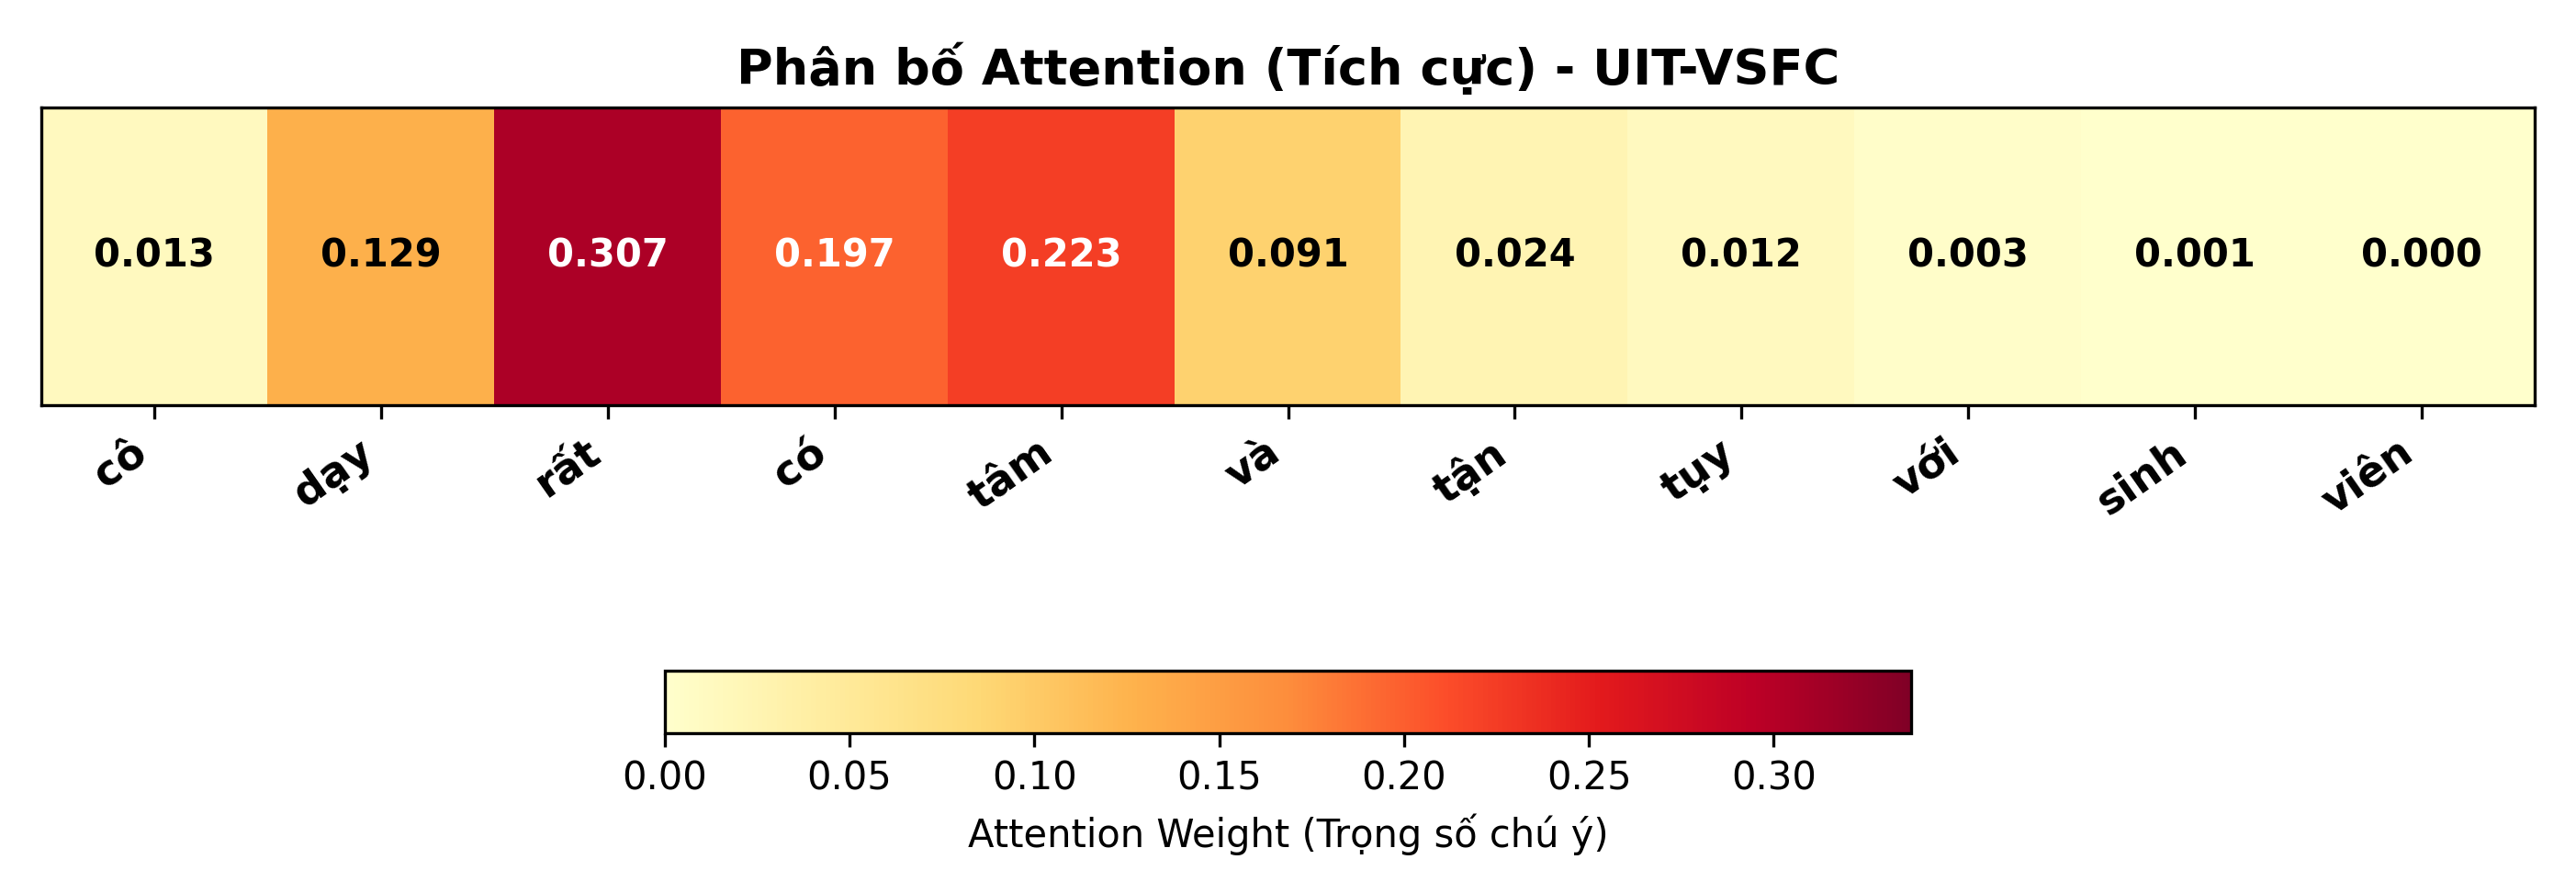
\includegraphics[width=0.96\textwidth]{images/attention_sample_pos.png}\\
      \vspace{0.08cm}
      {\fontsize{7}{8.5}\selectfont \textit{Hình: Mô hình tự động dồn trọng số vào từ quyết định.}}\\[0.15cm]
      \begin{alertblock}{Explainable AI (Khả năng giải thích)}
        \fontsize{7.5}{9}\selectfont
        Mô hình không còn là hộp đen bí ẩn. Nhìn vào $\alpha_t$, ta biết chính xác \textbf{vì sao máy tính dự đoán là Tích cực hay Tiêu cực}!
      \end{alertblock}
    \end{column}
  \end{columns}
\end{frame}

% ==================== PHẦN 7: TRANSFORMER & PHOBERT ====================
\begin{frame}{7. Bước Nhảy Vọt Lên Transformer \& PhoBERT Tiếng Việt SOTA}
  \begin{columns}[T, onlytextwidth]
    \begin{column}{0.50\textwidth}
      \begin{block}{Giới hạn của Word2Vec tĩnh}
        \fontsize{7.5}{9.5}\selectfont
        Word2Vec gán mỗi từ đúng 1 vector cố định:
        \begin{itemize}\setlength{\itemsep}{0.1em}
          \item \textit{''Tôi uống \textbf{nước} cam''} (chất lỏng).
          \item \textit{''Bảo vệ đất \textbf{nước}''} (quốc gia).
        \end{itemize}
        Cả hai từ \textit{''nước''} đều bị ép chung một tọa độ $\implies$ Sai lệch ngữ nghĩa!
      \end{block}
      \vspace{0.15cm}
      \begin{exampleblock}{Vai trò đại diện của token \texttt{[CLS]}}
        \fontsize{7.5}{9.5}\selectfont
        \begin{itemize}\setlength{\itemsep}{0.1em}
          \item Token đặc biệt \texttt{<s>} (\texttt{[CLS]}) đứng đầu câu.
          \item Nhờ \textbf{12 tầng Self-Attention}, \texttt{[CLS]} trực tiếp kết nối với mọi từ khác $\implies$ gom trọn ngữ nghĩa toàn câu vào 1 vector duy nhất $\mathbb{R}^{768}$!
        \end{itemize}
      \end{exampleblock}
    \end{column}
    \hfill
    \begin{column}{0.46\textwidth}
      \begin{alertblock}{Bí kíp trị Teencode: Tokenizer BPE}
        \fontsize{7.5}{9.5}\selectfont
        Khi gặp từ lóng hoặc viết tắt trên mạng:
        \begin{itemize}\setlength{\itemsep}{0.15em}
          \item Word2Vec tĩnh: Bó tay, gán thành từ rác \texttt{UNK} (Unknown).
          \item \textbf{PhoBERT (Byte-Pair Encoding)}: Tự động bẻ nhỏ từ lạ thành các mảnh âm tiết quen thuộc để suy luận.
        \end{itemize}
        $\implies$ Giúp PhoBERT đạt độ bền bỉ vượt trội trước ngôn ngữ mạng xã hội đầy nhiễu!
      \end{alertblock}
    \end{column}
  \end{columns}
\end{frame}

% ==================== PHẦN 8: BÀI TOÁN PHÂN LOẠI CẢM XÚC ====================
\begin{frame}{8. Thực Chiến: Bài Toán Phân Loại Cảm Xúc (Sentiment Analysis)}
  \fontsize{8}{10}\selectfont
  Để kiểm chứng các mô hình trên đời thực, nhóm tiến hành thử nghiệm trên \textbf{3 miền dữ liệu độc lập}:

  \vspace{0.15cm}
  \resizebox{\textwidth}{!}{
  \begin{tabular}{p{3.0cm}p{3.8cm}p{3.8cm}p{3.8cm}}
    \toprule
    \textbf{Đặc điểm} & \textbf{Miền 1: Giáo Dục (UIT-VSFC)} & \textbf{Miền 2: Mua Sắm (E-Commerce)} & \textbf{Miền 3: Điện Ảnh (Review Phim)} \\
    \midrule
    \textbf{Nội dung} & Khảo sát ý kiến sinh viên về giảng viên & Đánh giá chất lượng sản phẩm & Đánh giá diễn xuất, kịch bản phim \\
    \textbf{Phong cách} & Lịch sự, câu cú chuẩn ngữ pháp & Tiếng lóng, viết tắt, teencode (\textit{sp, ship, auth}) & Câu ghép dài, nhiều tương phản \\
    \textbf{Độ khó} & Trung bình (Dễ bắt từ khóa) & Rất cao (Nhiều nhiễu, lỗi chính tả, mỉa mai) & Cao (Khen diễn viên nhưng chê kịch bản) \\
    \bottomrule
  \end{tabular}
  }

  \vspace{0.2cm}
  \begin{columns}[T, onlytextwidth]
    \begin{column}{0.48\textwidth}
      \begin{block}{\small\textbf{Đầu vào (Input)}}
        \fontsize{8}{10}\selectfont
        Một đoạn văn bản nhận xét của người dùng (tiếng Việt hoặc tiếng Anh).
      \end{block}
    \end{column}
    \hfill
    \begin{column}{0.48\textwidth}
      \begin{block}{\small\textbf{Đầu ra (Output)}}
        \fontsize{8}{10}\selectfont
        Xác suất nhãn: \textbf{\color{HCMUEGreen}TÍCH CỰC} hay \textbf{\color{HCMUERed}TIÊU CỰC}.
      \end{block}
    \end{column}
  \end{columns}
\end{frame}

\begin{frame}{Bảng Đối Chuẩn Kết Quả: Ai Thắng Ai?}
  \fontsize{8}{10}\selectfont
  Kết quả thực nghiệm trên tập kiểm thử độc lập của 3 miền:

  \vspace{0.12cm}
  \resizebox{\textwidth}{!}{
  \begin{tabular}{clccc}
    \toprule
    \textbf{Cấp độ} & \textbf{Kiến trúc Mô hình} & \textbf{Giáo dục (UIT-VSFC)} & \textbf{TMĐT (E-Commerce)} & \textbf{Review Phim (IMDb)} \\
    \midrule
    \textbf{Cổ điển} & 1. TF-IDF + Logistic Regression & 89.83\% & 70.33\% & 89.20\% \\
    \textbf{Nhúng tĩnh} & 2. Average Word2Vec + Logistic Regression & 87.50\% & 67.33\% & 86.40\% \\
    \textbf{Chuỗi RNN} & 3. BiLSTM Classifier (Học từ đầu) & 89.17\% & 69.17\% & 88.10\% \\
    \textbf{Học chuyển giao} & 4. BiLSTM Pretrained Word2Vec & 91.00\% & 67.17\% & 90.80\% \\
    \textbf{Cơ chế Chú ý} & 5. BiLSTM + Self-Attention (\textbf{Đề xuất XAI}) & \textbf{\color{HCMUEDarkBlue}91.83\%} & \textbf{\color{HCMUEDarkBlue}72.50\%} & \textbf{\color{HCMUEDarkBlue}92.40\%} \\
    \textbf{Transformer SOTA} & 6. PhoBERT Base v2 (VinAI) & \textbf{\color{HCMUEGold}95.50\%} & \textbf{\color{HCMUEGold}86.17\%} & \textbf{\color{HCMUEGold}94.80\%} \\
    \bottomrule
  \end{tabular}
  }

  \vspace{0.2cm}
  \begin{columns}[T, onlytextwidth]
    \begin{column}{0.48\textwidth}
      \begin{block}{\small\textbf{Quan sát 1: Attention tạo bứt phá}}
        \fontsize{7.5}{9}\selectfont
        Tăng tới \textbf{+5.33\%} trên miền TMĐT nhờ khả năng lọc bỏ từ rác và bắt trúng từ cảm xúc.
      \end{block}
    \end{column}
    \hfill
    \begin{column}{0.48\textwidth}
      \begin{block}{\small\textbf{Quan sát 2: PhoBERT dẫn đầu toàn diện}}
        \fontsize{7.5}{9}\selectfont
        Đạt đỉnh \textbf{95.50\%} trên giáo dục và bền bỉ vượt trội trước tiếng lóng TMĐT (\textbf{86.17\%}).
      \end{block}
    \end{column}
  \end{columns}
\end{frame}

\begin{frame}{Khám Phá Trực Quan: Các Điểm Dữ Liệu Gom Nhóm Như Thế Nào?}
  \begin{columns}[c, onlytextwidth]
    \begin{column}{0.31\textwidth}
      \centering
      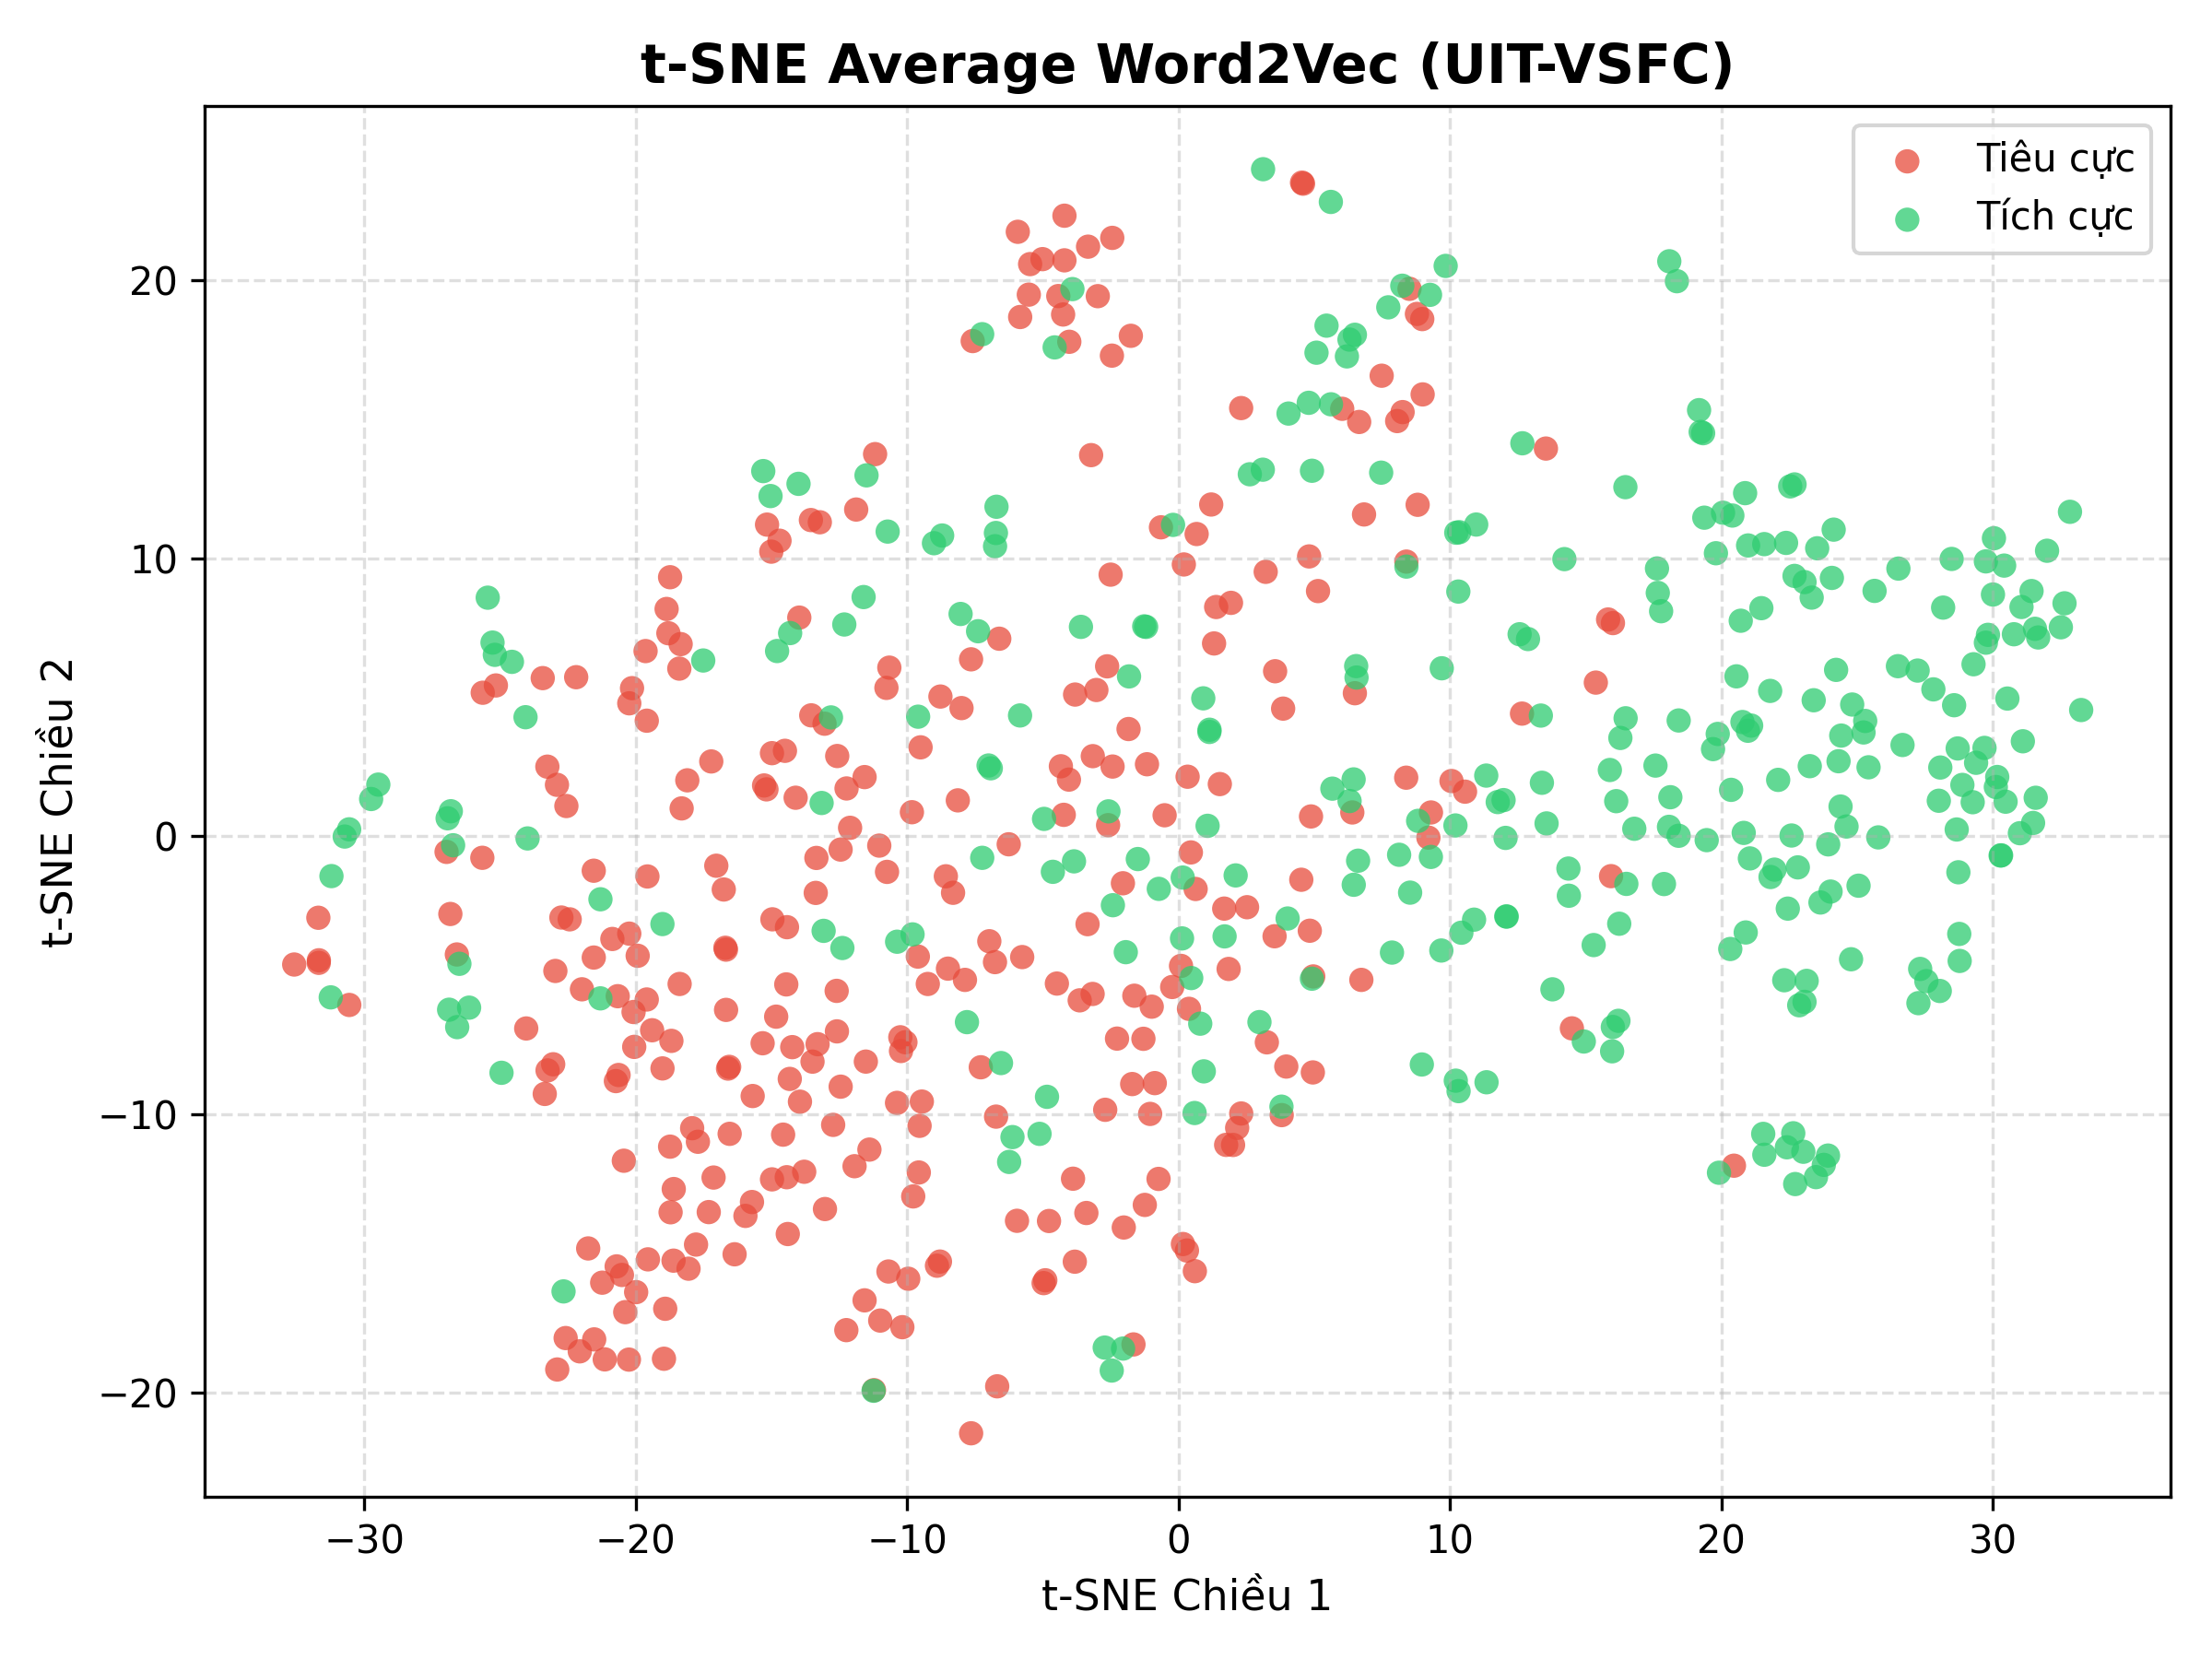
\includegraphics[width=\textwidth]{images/tsne_avg_word2vec.png}\\[0.2em]
      {\fontsize{7}{8.5}\selectfont \textbf{1. Average Word2Vec}\\Điểm đỏ (Neg) và xanh (Pos) dính chùm, ranh giới mờ nhạt.}
    \end{column}
    \hfill
    \begin{column}{0.31\textwidth}
      \centering
      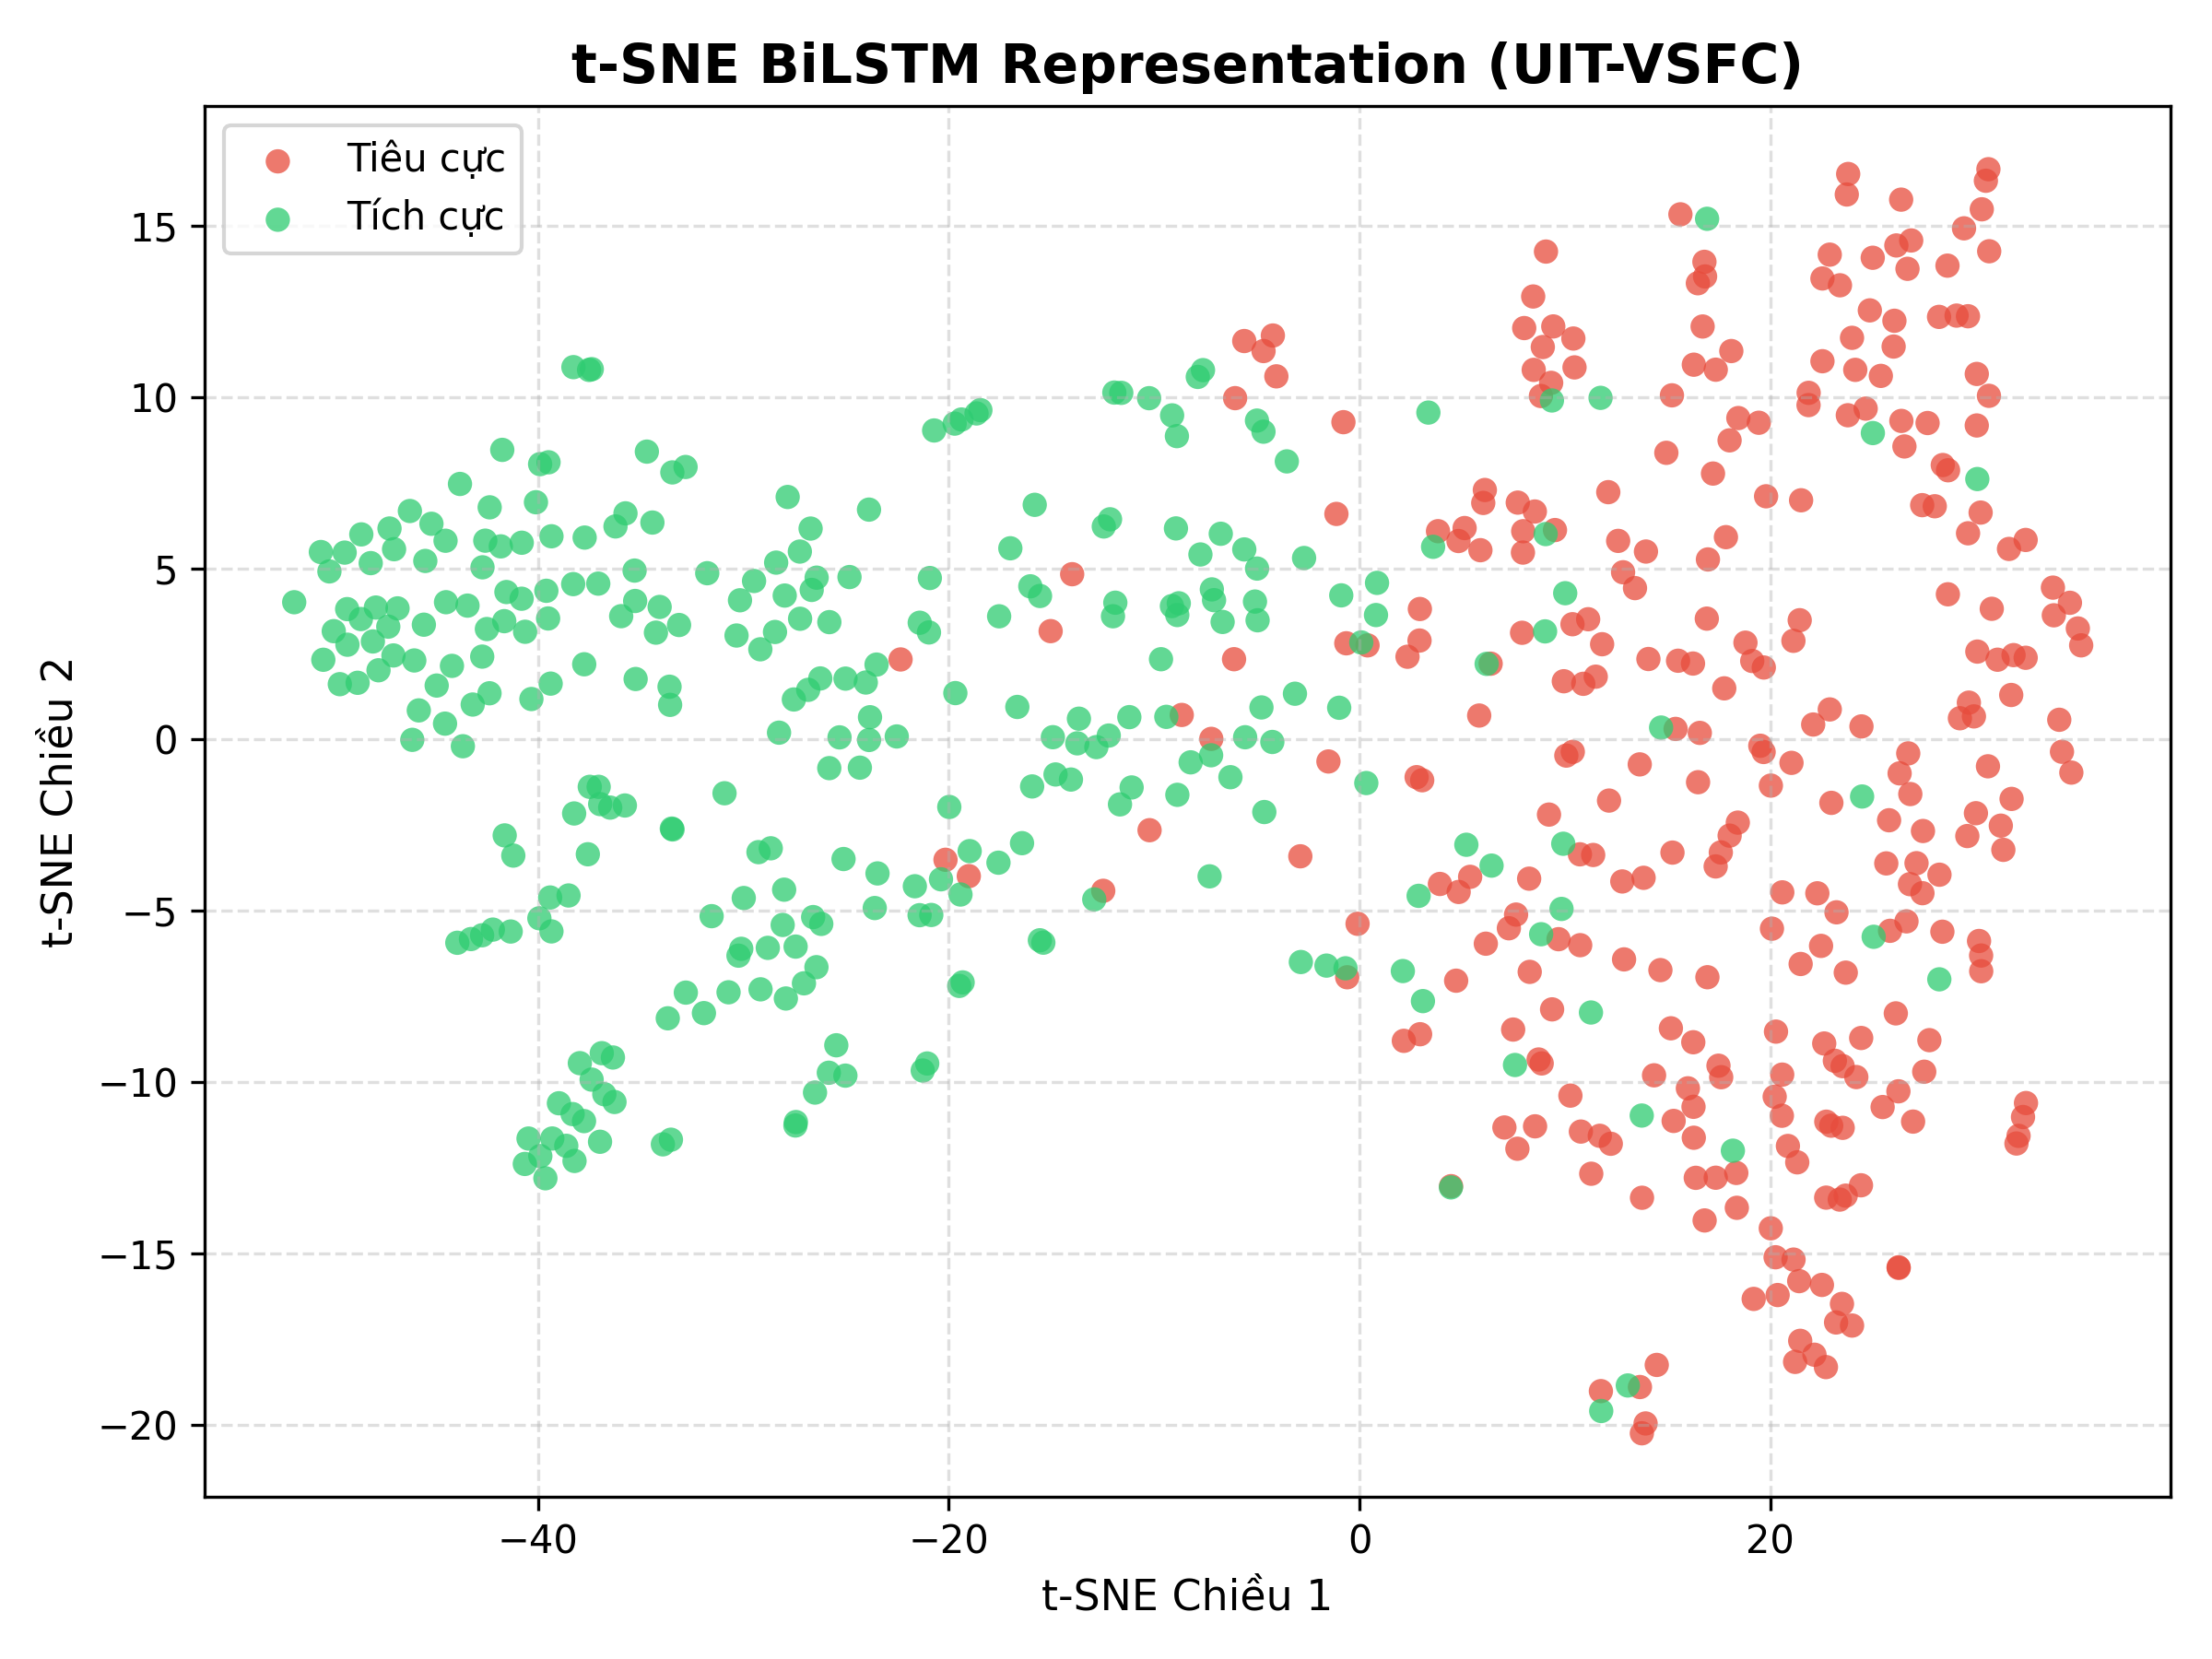
\includegraphics[width=\textwidth]{images/tsne_lstm_representation.png}\\[0.2em]
      {\fontsize{7}{8.5}\selectfont \textbf{2. BiLSTM Representation}\\Bắt đầu tách thành 2 nhánh rõ ràng nhờ học chuỗi.}
    \end{column}
    \hfill
    \begin{column}{0.31\textwidth}
      \centering
      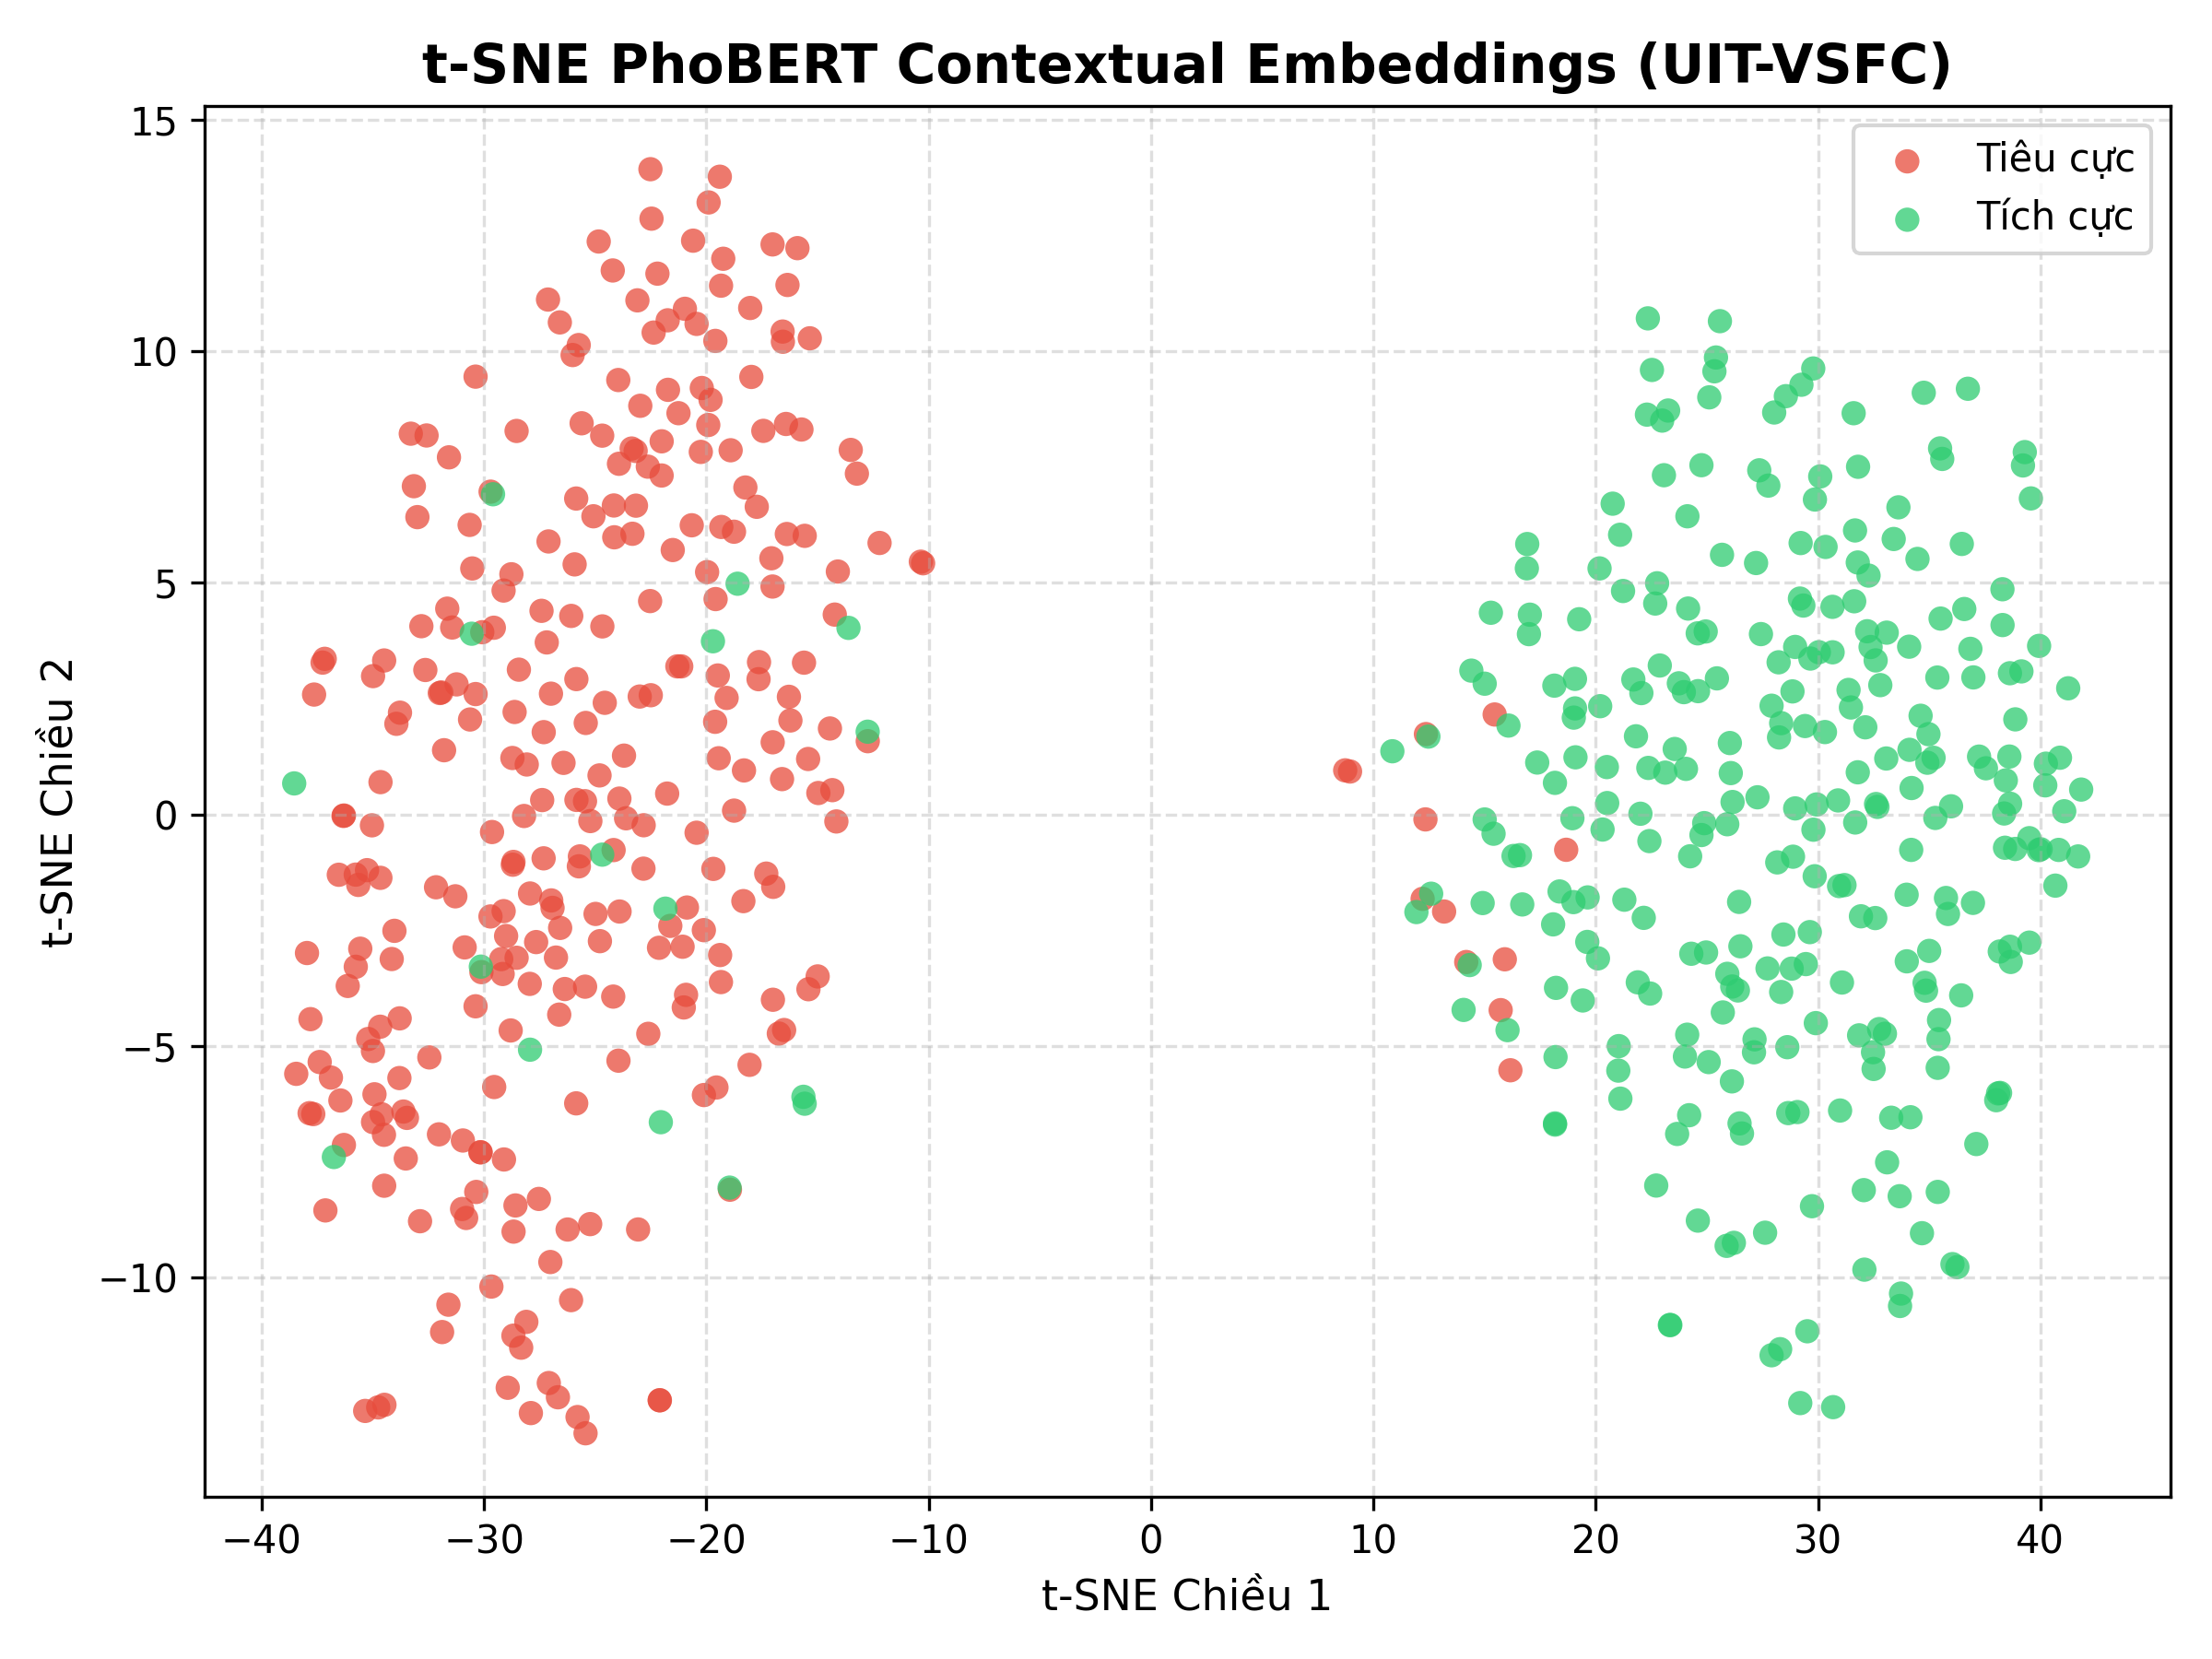
\includegraphics[width=\textwidth]{images/tsne_phobert_representation.png}\\[0.2em]
      {\fontsize{7}{8.5}\selectfont \textbf{3. PhoBERT Contextual}\\Tách biệt tuyệt đối thành 2 khối tách rời nhau!}
    \end{column}
  \end{columns}

  \vspace{0.25cm}
  \begin{block}{\small\textbf{Ý nghĩa trực quan}}
    \fontsize{8}{10.5}\selectfont
    Mô hình càng xịn thì không gian biểu diễn càng tách bạch rõ ràng giữa \textbf{Vui (Tích cực)} và \textbf{Buồn (Tiêu cực)}, giúp việc kẻ một đường phân cách trở nên dễ dàng và chuẩn xác!
  \end{block}
\end{frame}

\begin{frame}{Các Ca Khó Kinh Điển Trong Đời Thực \& Giải Pháp Kỹ Thuật}
  \begin{columns}[T, onlytextwidth]
    \begin{column}{0.48\textwidth}
      \begin{block}{Ca 1: Cấu trúc câu tương phản ("...nhưng...")}
        \fontsize{7.5}{9.5}\selectfont
        \begin{itemize}\setlength{\itemsep}{0.15em}
          \item \textbf{Câu mẫu}: \textit{''Giao hàng hơi lâu nhưng chất lượng áo đỉnh chóp.''} $\to$ \textbf{TÍCH CỰC}.
          \item \textbf{Thách thức}: Từ lóng lạ + từ tiêu cực ở đầu câu.
        \end{itemize}
        \vspace{0.08cm}
        \textbf{\color{HCMUEDarkBlue}$\implies$ Hướng khắc phục}:
        \begin{itemize}\fontsize{7}{8.5}\selectfont\setlength{\itemsep}{0.1em}
          \item Tách vế câu qua liên từ nghịch tiếp (\textit{nhưng, tuy nhiên}) để xét trọng số riêng cho vế kết luận.
          \item Bổ sung từ điển chuẩn hóa Teencode tự động.
        \end{itemize}
      \end{block}
    \end{column}
    \hfill
    \begin{column}{0.48\textwidth}
      \begin{alertblock}{Ca 2: Mỉa mai, châm biếm (Sarcasm)}
        \fontsize{7.5}{9.5}\selectfont
        \begin{itemize}\setlength{\itemsep}{0.15em}
          \item \textbf{Câu mẫu}: \textit{''Shop quá nhiệt tình, nhắn tin 3 ngày mới thèm rep.''} $\to$ \textbf{TIÊU CỰC}.
          \item \textbf{Thách thức}: Khen bề mặt chữ nhưng ngụ ý chê.
        \end{itemize}
        \vspace{0.08cm}
        \textbf{\color{HCMUERed}$\implies$ Hướng khắc phục}:
        \begin{itemize}\fontsize{7}{8.5}\selectfont\setlength{\itemsep}{0.1em}
          \item Bổ sung Đồ thị tri thức (Knowledge Graph): \textit{''3 ngày''} là sự cố trễ hạn nghiêm trọng.
          \item Áp dụng mô hình suy luận chuỗi tư duy (Chain-of-Thought) của các mô hình ngôn ngữ lớn (LLMs).
        \end{itemize}
      \end{alertblock}
    \end{column}
  \end{columns}
\end{frame}

% ==================== PHẦN 9: TỔNG KẾT & LỜI KHUYÊN ====================
\begin{frame}{9. Trải Nghiệm Thực Tế Hệ Thống Web Demo}
  \begin{columns}[c, onlytextwidth]
    \begin{column}{0.48\textwidth}
      \begin{block}{Học đi đôi với hành (Interactive Demo)}
        \fontsize{7.5}{9.5}\selectfont
        Nhóm đã xây dựng sẵn một ứng dụng Web trực quan:
        \begin{itemize}\setlength{\itemsep}{0.15em}
          \item \textbf{Gõ câu bất kỳ}: Tiếng Việt hoặc tiếng Anh, có teencode, viết tắt.
          \item \textbf{So sánh 6 mô hình cùng lúc}: Xem mô hình nào đoán đúng, mô hình nào bị lừa.
          \item \textbf{Xem bản đồ nhiệt Attention}: Rê chuột xem trọng số $\alpha_t$ của từng từ.
        \end{itemize}
      \end{block}
      \vspace{0.15cm}
      \begin{exampleblock}{Khởi chạy đơn giản với 1 câu lệnh}
        \fontsize{7.5}{9.5}\selectfont
        \texttt{cd Bai\_tap\_giua\_ky \&\& ./run\_app.sh}
      \end{exampleblock}
    \end{column}
    \hfill
    \begin{column}{0.48\textwidth}
      \centering
      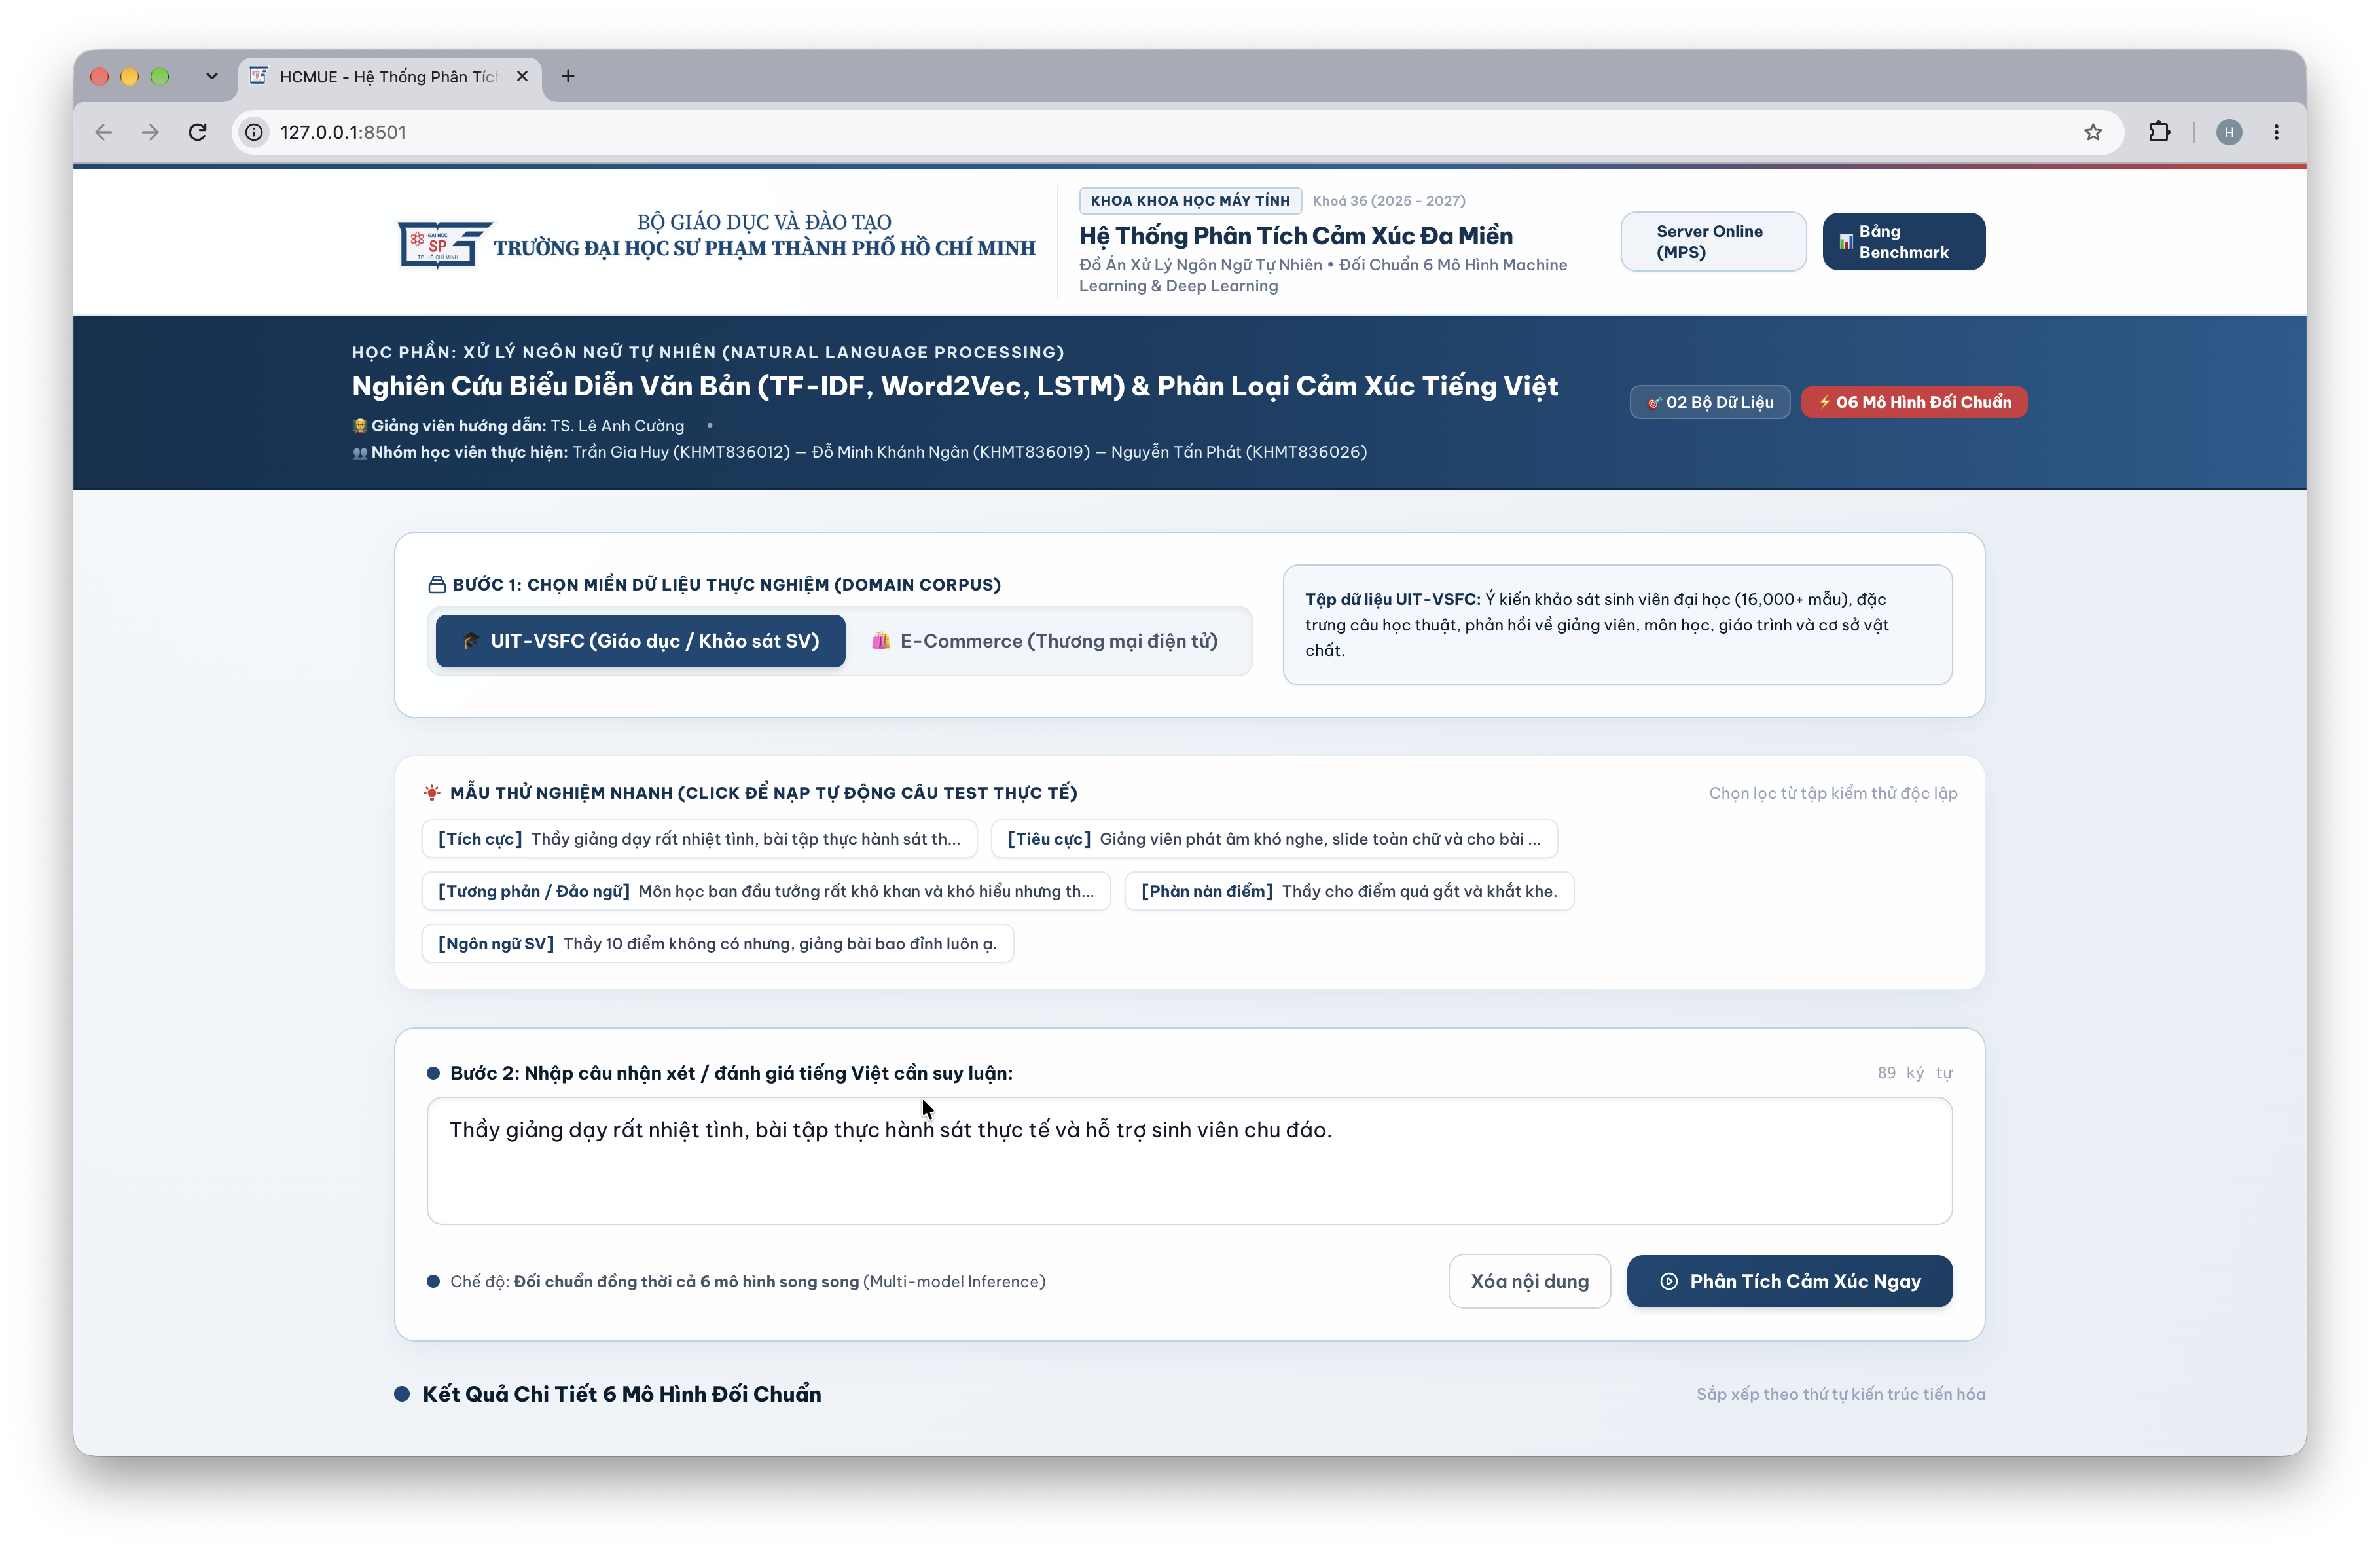
\includegraphics[width=0.96\textwidth]{images/demo_overview.png}\\
      \vspace{0.08cm}
      {\fontsize{7}{8.5}\selectfont \textit{Hình: Giao diện trực quan hoá 6 mô hình đối đầu.}}
    \end{column}
  \end{columns}
\end{frame}

\begin{frame}{Tổng Kết: 5 Bài Học Cốt Lõi Cho Người Mới Bắt Đầu}
  \begin{columns}[T, onlytextwidth]
    \begin{column}{0.48\textwidth}
      \begin{block}{\small\textbf{1. Biểu diễn từ là nền tảng}}
        \fontsize{7.5}{9.5}\selectfont
        Không có vector chất lượng, không mô hình nào tốt. Từ One-Hot rời rạc $\to$ Word2Vec là bước ngoặt vĩ đại của NLP.
      \end{block}
      \vspace{0.15cm}
      \begin{block}{\small\textbf{2. Trật tự câu quyết định ý nghĩa}}
        \fontsize{7.5}{9.5}\selectfont
        Đừng chỉ cộng trung bình các từ. Hãy dùng \textbf{BiLSTM} để giữ trọn ngữ cảnh hai chiều xuôi - ngược.
      \end{block}
      \vspace{0.15cm}
      \begin{block}{\small\textbf{3. Cơ chế Chú ý mở toang hộp đen}}
        \fontsize{7.5}{9.5}\selectfont
        \textbf{Self-Attention} vừa tăng độ chính xác vừa cho biết lý do AI đưa ra quyết định (\textbf{XAI}).
      \end{block}
    \end{column}
    \hfill
    \begin{column}{0.48\textwidth}
      \begin{block}{\small\textbf{4. Transformer là tương lai}}
        \fontsize{7.5}{9.5}\selectfont
        Mô hình lớn như \textbf{PhoBERT} giải quyết đa nghĩa và bền bỉ trước tiếng lóng nhờ Tokenizer BPE.
      \end{block}
      \vspace{0.15cm}
      \begin{exampleblock}{\small\textbf{5. Dữ liệu quan trọng hơn mô hình}}
        \fontsize{7.5}{9.5}\selectfont
        Mô hình 95\% ở giáo dục có thể tụt xuống 72\% ở TMĐT do sự dịch chuyển phân phối (\textbf{Domain Gap}).
      \end{exampleblock}
    \end{column}
  \end{columns}
\end{frame}

% ==================== SLIDE CUỐI: CẢM ƠN & Q&A ====================
{
\setbeamertemplate{background}{}
\setbeamertemplate{footline}{}
\setbeamertemplate{frametitle}{}
\begin{frame}[plain]
  \begin{tikzpicture}[remember picture,overlay]
    \fill[HCMUEDarkBlue] (current page.north west) rectangle (current page.south east);
    
    % Nền mờ Tòa nhà A-01 chuẩn HCMUE_PPT Template.pptx
    \node[anchor=south east, inner sep=0pt] at ($(current page.south east)+(0, 0)$) {
      
\includegraphics[width=9.5cm]{images/toa_nha_a_watermark_dark.png}
    };
    
    \fill[HCMUECerulean!25] ($(current page.south east)+(-2,2)$) circle (3.5cm);
    \fill[HCMUECerulean!15] ($(current page.north west)+(3,-2)$) circle (2.5cm);
  \end{tikzpicture}

  \begin{center}
    % Logo kèm chữ chính thức phiên bản chữ trắng nổi bật trên nền xanh đậm
    
\includegraphics[height=1.35cm]{images/logo_hcmue_kemchu_eng_white.png}

    \vspace{0.4em}
    {\fontsize{10.5}{13}\selectfont \textbf{\color{white!90}KHOA CÔNG NGHỆ THÔNG TIN — LỚP CAO HỌC KHMT K36}}\\[0.8em]

    {\fontsize{18}{22}\selectfont \textbf{\color{HCMUEGold}CẢM ƠN CÁC BẠN ĐÃ THEO DÕI BÀI GIẢNG!}}\\[0.3em]
    {\fontsize{13}{16}\selectfont \textbf{\color{white}CHÚC CÁC BẠN CHINH PHỤC THÀNH CÔNG NLP!}}\\[0.7em]

    \begin{beamercolorbox}[wd=0.72\textwidth,rounded=true,center,sep=0.35em]{palette secondary}
      \fontsize{9.5}{12}\selectfont
      \textbf{Giảng viên hướng dẫn: PGS.TS. LÊ ANH CƯỜNG}\\[0.2em]
      \fontsize{8.5}{11}\selectfont
      Nhóm 3: Trần Gia Huy $\bullet$ Đỗ Minh Khánh Ngân $\bullet$ Nguyễn Tấn Phát
    \end{beamercolorbox}

    \vspace{0.4em}
    {\fontsize{10.5}{13}\selectfont \textbf{\color{white}GÓC THẢO LUẬN \& GIẢI ĐÁP THẮC MẮC (Q\&A)}}\\[0.15em]
    {\fontsize{8}{10}\selectfont \color{white!70}Mã nguồn bài học \& Web Demo: \url{https://github.com/trangiahuy8444/NLP}}
  \end{center}
\end{frame}
}

\end{document}
